\chapter*{Spis załączników}
\addcontentsline{toc}{chapter}{Spis załączników}
\noindent

\begin{tabularx}{\textwidth}{Xl}

    Pełny schemat bazy danych & str. \pageref{file:database-schema} \\

    Pełny opis zadania projektowego dla przedmiotu ”Podstawy Programowania” w realizacji zima 2018 & str. \pageref{file:penguins_description} \\

    Definicja przypadków testowych dla symulacji projektu historycznego & str. \pageref{file:test_cases_penguins} \\

    Definicja przypadków testowych dla symulacji projektu z operacjami na macierzach & str. \pageref{file:test_cases_matrix} \\

\end{tabularx}

\chapter*{Załączniki}
\addcontentsline{toc}{chapter}{Załączniki}

%%%%%%%%%%%%%%%%%%%%%%%%%%%%%%%%%%%%%%%%%%%%%%%%%%%%%%%%%%%%%%%%%%%%%%%%%%
\section*{Pełny schemat bazy danych}
\label{file:database-schema}
{
\tiny
\verbatiminput{back//platform_schema.sql}
}

%%%%%%%%%%%%%%%%%%%%%%%%%%%%%%%%%%%%%%%%%%%%%%%%%%%%%%%%%%%%%%%%%%%%%%%%%%
\section*{Pełny opis zadania projektowego dla przedmiotu ”Podstawy Programowania” w realizacji zima 2018}
\label{file:penguins_description}
{
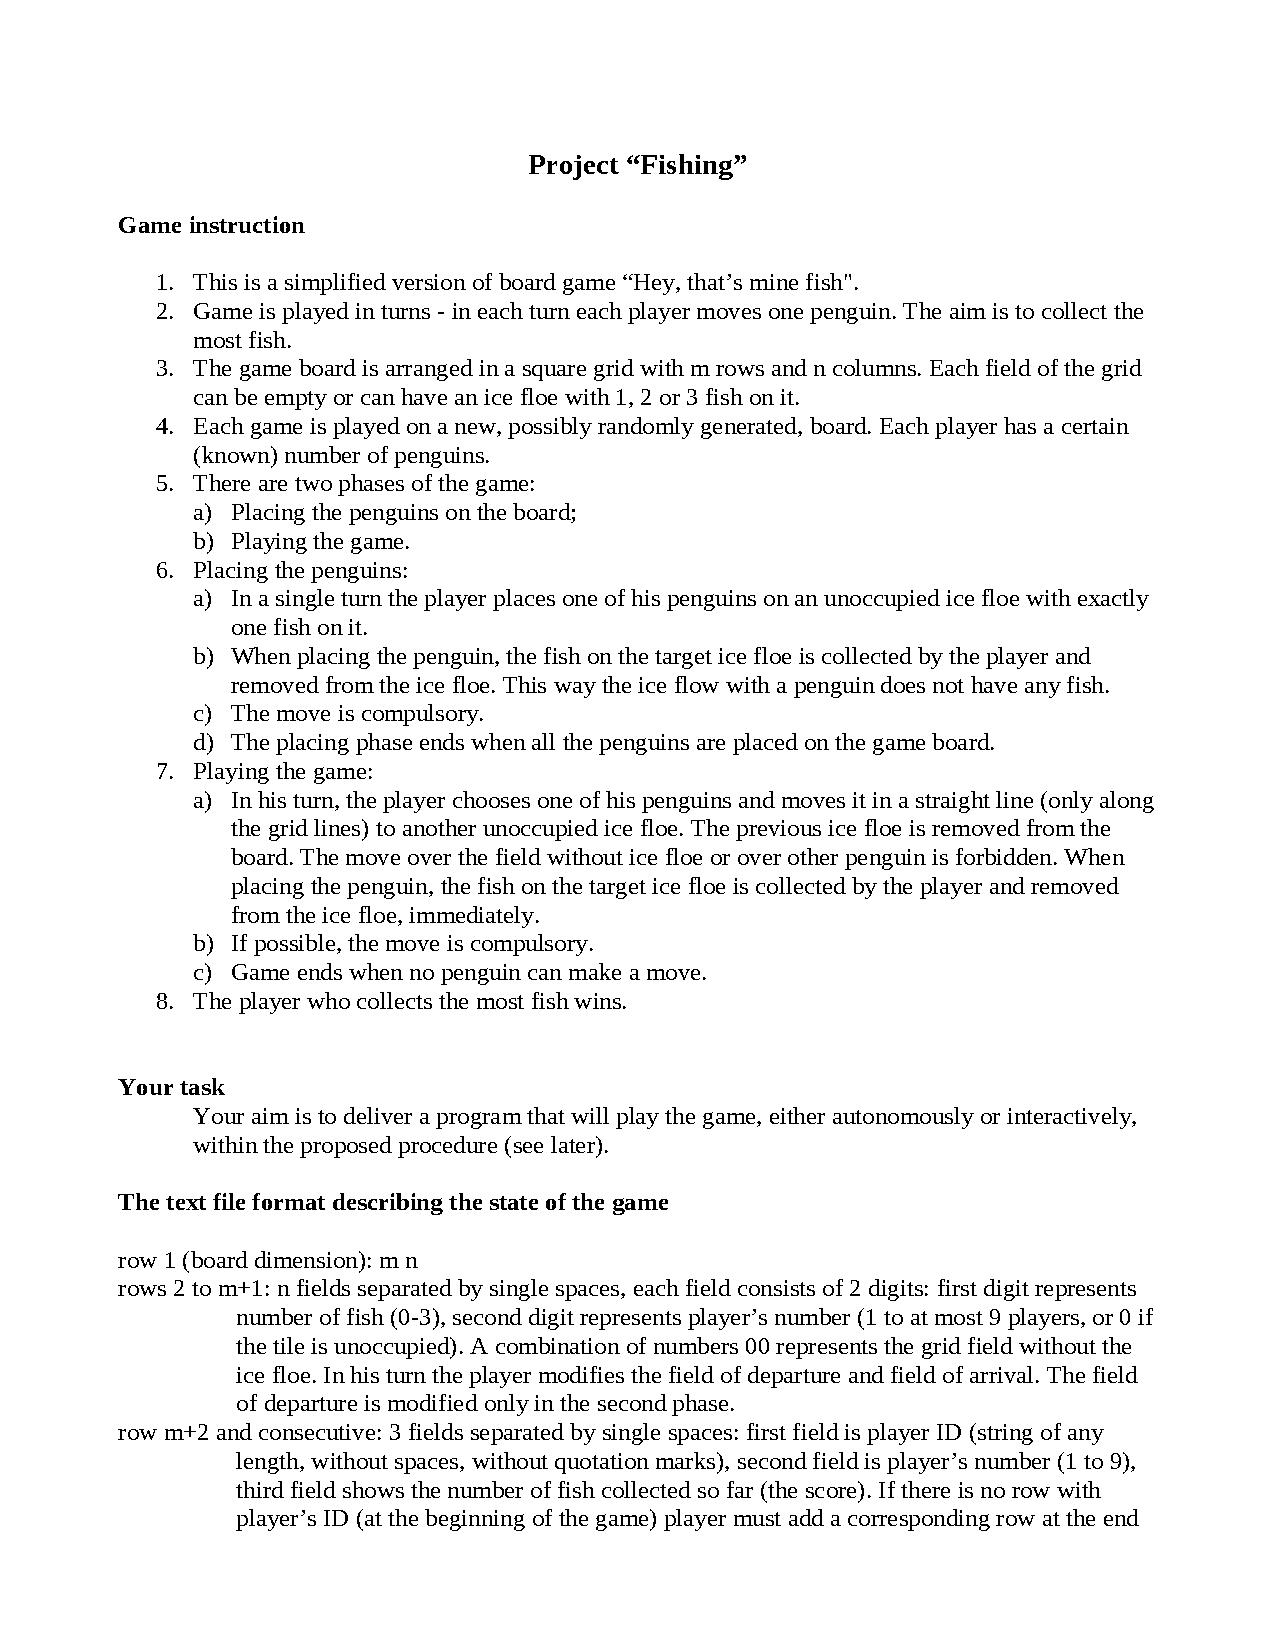
\includepdf[page={1,2,3,4}]{back//penguins_description}
}


%%%%%%%%%%%%%%%%%%%%%%%%%%%%%%%%%%%%%%%%%%%%%%%%%%%%%%%%%%%%%%%%%%%%%%%%%%
\section*{Definicja przypadków testowych dla symulacji zmodyfikowanego projektu historycznego}
\label{file:test_cases_penguins}

{
\setlength\parindent{0pt}

\large
\textbf{Etap: \textit{Read parse write}}
\normalsize

\textbf{Nazwa testu: \textit{Invalid input file}}

\begin{table}[H]
    \centering
    \caption{Definicja przypadku testowego \textit{Invalid input file}}
    \scalebox{0.65}{
    \begin{tabular}{|l|l|l|}
        \hline
        \rowcolor[HTML]{EFEFEF}
        Plik wejściowy & Parametry & Oczekiwany plik wyjściowy \\ \hline
        \pbox{20cm}{
        \vspace{.5\baselineskip}
        10 10 \\
        30 30 30 01 20 30 20 20 10 20 \\
        20 03 10 01 00 03 10 20 10 10 \\
        10 01 10 20 20 10 03 10 30 02 \\
        30 20 30 20 10 30 30 30 30 20 \\
        30 30 30 10 30 30 10 30 10 \\
        30 30 30 10 30 30 10 10 30 20 \\
        30 20 20 30 30 30 20 30 10 02 \\
        20 20 20 30 20 20 10 01 20 20 \\
        02 20 30 30 20 30 10 10 30 01 \\
        10 30 10 10 10 30 10 10 30 30 \\
        TEAM1 1 0 \\
        team2 2 0 \\
        Team3 3 0
        \vspace{.5\baselineskip} }            & Brak & Invalid input file                         \\ \hline
    \end{tabular}
    }
\end{table}


\textbf{Nazwa testu: \textit{Read parse write}}

\begin{table}[H]
    \centering
    \caption{Definicja przypadku testowego \textit{Read parse write}}
    \scalebox{0.65}{
    \begin{tabular}{|l|l|l|}
        \hline
        \rowcolor[HTML]{EFEFEF}
        Plik wejściowy & Parametry & Oczekiwany plik wyjściowy \\ \hline
        \pbox{20cm}{
        \vspace{.5\baselineskip}
        10 10 \\
        30 30 30 01 20 30 20 20 10 20 \\
        20 03 10 01 00 03 10 20 10 10 \\
        10 01 10 20 20 10 03 10 30 02 \\
        30 20 30 20 10 30 30 30 30 20 \\
        30 30 30 10 30 30 10 30 10 20 \\
        30 30 30 10 30 30 10 10 30 20 \\
        30 20 20 30 30 30 20 30 10 02 \\
        20 20 20 30 20 20 10 01 20 20 \\
        02 20 30 30 20 30 10 10 30 01 \\
        10 30 10 10 10 30 10 10 30 30 \\
        TEAM1 1 0 \\
        team2 2 0 \\
        Team3 3 0
        \vspace{.5\baselineskip} }     &
        Brak &
        \pbox{20cm}{
        \vspace{.5\baselineskip}
        10 10 \\
        30 30 30 01 20 30 20 20 10 20 \\
        20 03 10 01 00 03 10 20 10 10 \\
        10 01 10 20 20 10 03 10 30 02 \\
        30 20 30 20 10 30 30 30 30 20 \\
        30 30 30 10 30 30 10 30 10 20 \\
        30 30 30 10 30 30 10 10 30 20 \\
        30 20 20 30 30 30 20 30 10 02 \\
        20 20 20 30 20 20 10 01 20 20 \\
        02 20 30 30 20 30 10 10 30 01 \\
        10 30 10 10 10 30 10 10 30 30 \\
        TEAM1 1 0 \\
        team2 2 0 \\
        Team3 3 0
        \vspace{.5\baselineskip} }                         \\ \hline
    \end{tabular}
    }
\end{table}

\large
\textbf{Etap: \textit{Set penguins}}
\normalsize

\textbf{Nazwa testu: \textit{Place on cell with too many fish}}

\begin{table}[H]
    \centering
    \caption{Definicja przypadku testowego \textit{Place on cell with too many fish}}
    \scalebox{0.65}{
    \begin{tabular}{|l|l|l|}
        \hline
        \rowcolor[HTML]{EFEFEF}
        Plik wejściowy & Parametry & Oczekiwany plik wyjściowy \\ \hline
        \pbox{20cm}{
        \vspace{.5\baselineskip}
        10 10 \\
        30 30 30 01 20 30 20 20 10 20 \\
        20 03 10 01 00 03 10 20 10 10 \\
        10 01 10 20 20 10 03 10 30 02 \\
        30 20 30 20 10 30 30 30 30 20 \\
        30 30 30 10 30 30 10 30 10 20 \\
        30 30 30 10 30 30 10 10 30 20 \\
        30 20 20 30 30 30 20 30 10 02 \\
        20 20 20 30 20 20 10 01 20 20 \\
        02 20 30 30 20 30 10 10 30 01 \\
        10 30 10 10 10 30 10 10 30 30 \\
        TEAM1 1 0 \\
        team2 2 0 \\
        Team3 3 0
        \vspace{.5\baselineskip} }            &
        \pbox{20cm}{
        \vspace{.5\baselineskip}
        id=1 \\
        phase=placement \\
        placement\_x=0 \\
        placement\_y=0
        \vspace{.5\baselineskip} } &
        Invalid parameters                         \\ \hline
    \end{tabular}
    }
\end{table}



\textbf{Nazwa testu: \textit{Place outside of board}}

\begin{table}[H]
    \centering
    \caption{Definicja przypadku testowego \textit{Place outside of board}}
    \scalebox{0.65}{
    \begin{tabular}{|l|l|l|}
        \hline
        \rowcolor[HTML]{EFEFEF}
        Plik wejściowy & Parametry & Oczekiwany plik wyjściowy \\ \hline
        \pbox{20cm}{
        \vspace{.5\baselineskip}
        10 10 \\
        30 30 30 01 20 30 20 20 10 20 \\
        20 03 10 01 00 03 10 20 10 10 \\
        10 01 10 20 20 10 03 10 30 02 \\
        30 20 30 20 10 30 30 30 30 20 \\
        30 30 30 10 30 30 10 30 10 20 \\
        30 30 30 10 30 30 10 10 30 20 \\
        30 20 20 30 30 30 20 30 10 02 \\
        20 20 20 30 20 20 10 01 20 20 \\
        02 20 30 30 20 30 10 10 30 01 \\
        10 30 10 10 10 30 10 10 30 30 \\
        TEAM1 1 0 \\
        team2 2 0 \\
        Team3 3 0
        \vspace{.5\baselineskip} }            &
        \pbox{20cm}{
        \vspace{.5\baselineskip}
        id=2 \\
        phase=placement \\
        placement\_x=13 \\
        placement\_y=4
        \vspace{.5\baselineskip} } &
        Invalid parameters                         \\ \hline
    \end{tabular}
    }
\end{table}

\pagebreak

\textbf{Nazwa testu: \textit{Place player 2 on 3 4}}

\begin{table}[H]
    \centering
    \caption{Definicja przypadku testowego \textit{Place player 2 on 3 4}}
    \scalebox{0.65}{
    \begin{tabular}{|l|l|l|}
        \hline
        \rowcolor[HTML]{EFEFEF}
        Plik wejściowy & Parametry & Oczekiwany plik wyjściowy \\ \hline
        \pbox{20cm}{
        \vspace{.5\baselineskip}
        10 10 \\
        30 30 30 01 20 30 20 20 10 20 \\
        20 03 10 01 00 03 10 20 10 10 \\
        10 01 10 20 20 10 03 10 30 02 \\
        30 20 30 20 10 30 30 30 30 20 \\
        30 30 30 10 30 30 10 30 10 20 \\
        30 30 30 10 30 30 10 10 30 20 \\
        30 20 20 30 30 30 20 30 10 02 \\
        20 20 20 30 20 20 10 01 20 20 \\
        02 20 30 30 20 30 10 10 30 01 \\
        10 30 10 10 10 30 10 10 30 30 \\
        TEAM1 1 0 \\
        team2 2 0 \\
        Team3 3 0
        \vspace{.5\baselineskip} }            &
        \pbox{20cm}{
        \vspace{.5\baselineskip}
        id=2 \\
        phase=placement \\
        placement\_x=3 \\
        placement\_y=4
        \vspace{.5\baselineskip} } &
        \pbox{20cm}{
        \vspace{.5\baselineskip}
        10 10 \\
        30 30 30 01 20 30 20 20 10 20 \\
        20 03 10 01 00 03 10 20 10 10 \\
        10 01 10 20 20 10 03 10 30 02 \\
        30 20 30 20 10 30 30 30 30 20 \\
        30 30 30 02 30 30 10 30 10 20 \\
        30 30 30 10 30 30 10 10 30 20 \\
        30 20 20 30 30 30 20 30 10 02 \\
        20 20 20 30 20 20 10 01 20 20 \\
        02 20 30 30 20 30 10 10 30 01 \\
        10 30 10 10 10 30 10 10 30 30 \\
        TEAM1 1 0 \\
        team2 2 1 \\
        Team3 3 0
        \vspace{.5\baselineskip} } \\ \hline
    \end{tabular}
    }
\end{table}



\textbf{Nazwa testu: \textit{Place with player id too high}}

\begin{table}[H]
    \centering
    \caption{Definicja przypadku testowego \textit{Place with player id too high}}
    \scalebox{0.65}{
    \begin{tabular}{|l|l|l|}
        \hline
        \rowcolor[HTML]{EFEFEF}
        Plik wejściowy & Parametry & Oczekiwany plik wyjściowy \\ \hline
        \pbox{20cm}{
        \vspace{.5\baselineskip}
        10 10 \\
        30 30 30 01 20 30 20 20 10 20 \\
        20 03 10 01 00 03 10 20 10 10 \\
        10 01 10 20 20 10 03 10 30 02 \\
        30 20 30 20 10 30 30 30 30 20 \\
        30 30 30 10 30 30 10 30 10 20 \\
        30 30 30 10 30 30 10 10 30 20 \\
        30 20 20 30 30 30 20 30 10 02 \\
        20 20 20 30 20 20 10 01 20 20 \\
        02 20 30 30 20 30 10 10 30 01 \\
        10 30 10 10 10 30 10 10 30 30 \\
        TEAM1 1 0 \\
        team2 2 0 \\
        Team3 3 0
        \vspace{.5\baselineskip} }            &
        \pbox{20cm}{
        \vspace{.5\baselineskip}
        id=5 \\
        phase=placement \\
        placement\_x=3 \\
        placement\_y=4
        \vspace{.5\baselineskip} } &
        Invalid parameters                         \\ \hline
    \end{tabular}
    }
\end{table}

\pagebreak

\large
\textbf{Etap: \textit{Move penguins}}
\normalsize

\textbf{Nazwa testu: \textit{Move penguin 1 1 down to other penguin}}

\begin{table}[H]
    \centering
    \caption{Definicja przypadku testowego \textit{Move penguin 1 1 down to other penguin}}
    \scalebox{0.65}{
    \begin{tabular}{|l|l|l|}
        \hline
        \rowcolor[HTML]{EFEFEF}
        Plik wejściowy & Parametry & Oczekiwany plik wyjściowy \\ \hline
        \pbox{20cm}{
        \vspace{.5\baselineskip}
        10 10 \\
        30 30 30 01 20 30 20 20 10 20 \\
        20 03 10 01 00 03 10 20 10 10 \\
        10 01 10 20 20 10 03 10 30 02 \\
        30 20 30 20 10 30 30 30 30 20 \\
        30 30 30 10 30 30 10 30 10 20 \\
        30 30 30 10 30 30 10 10 30 20 \\
        30 20 20 30 30 30 20 30 10 02 \\
        20 20 20 30 20 20 10 01 20 20 \\
        02 20 30 30 20 30 10 10 30 01 \\
        10 30 10 10 10 30 10 10 30 30 \\
        TEAM1 1 0 \\
        team2 2 0 \\
        Team3 3 0
        \vspace{.5\baselineskip} }            &
        \pbox{20cm}{
        \vspace{.5\baselineskip}
        id=3 \\
        phase=move \\
        from\_x=1 \\
        from\_y=1 \\
        direction=down
        \vspace{.5\baselineskip} } &
        Invalid parameters                         \\ \hline
    \end{tabular}
    }
\end{table}



\textbf{Nazwa testu: \textit{Move penguin 1 1 up}}

\begin{table}[H]
    \centering
    \caption{Definicja przypadku testowego \textit{Move penguin 1 1 up}}
    \scalebox{0.65}{
    \begin{tabular}{|l|l|l|}
        \hline
        \rowcolor[HTML]{EFEFEF}
        Plik wejściowy & Parametry & Oczekiwany plik wyjściowy \\ \hline
        \pbox{20cm}{
        \vspace{.5\baselineskip}
        10 10 \\
        30 30 30 01 20 30 20 20 10 20 \\
        20 03 10 01 00 03 10 20 10 10 \\
        10 01 10 20 20 10 03 10 30 02 \\
        30 20 30 20 10 30 30 30 30 20 \\
        30 30 30 10 30 30 10 30 10 20 \\
        30 30 30 10 30 30 10 10 30 20 \\
        30 20 20 30 30 30 20 30 10 02 \\
        20 20 20 30 20 20 10 01 20 20 \\
        02 20 30 30 20 30 10 10 30 01 \\
        10 30 10 10 10 30 10 10 30 30 \\
        TEAM1 1 0 \\
        team2 2 0 \\
        Team3 3 0
        \vspace{.5\baselineskip} }            &
        \pbox{20cm}{
        \vspace{.5\baselineskip}
        id=3 \\
        phase=move \\
        from\_x=1 \\
        from\_y=1 \\
        direction=up
        \vspace{.5\baselineskip} } &
        \pbox{20cm}{
        \vspace{.5\baselineskip}
        10 10 \\
        30 03 30 01 20 30 20 20 10 20 \\
        20 00 10 01 00 03 10 20 10 10 \\
        10 01 10 20 20 10 03 10 30 02 \\
        30 20 30 20 10 30 30 30 30 20 \\
        30 30 30 10 30 30 10 30 10 20 \\
        30 30 30 10 30 30 10 10 30 20 \\
        30 20 20 30 30 30 20 30 10 02 \\
        20 20 20 30 20 20 10 01 20 20 \\
        02 20 30 30 20 30 10 10 30 01 \\
        10 30 10 10 10 30 10 10 30 30 \\
        TEAM1 1 0 \\
        team2 2 0 \\
        Team3 3 3
        \vspace{.5\baselineskip}
        } \\ \hline
    \end{tabular}
    }
\end{table}

\pagebreak

\textbf{Nazwa testu: \textit{Move penguin 3 1 right to empty}}

\begin{table}[H]
    \centering
    \caption{Definicja przypadku testowego \textit{Move penguin 3 1 right to empty}}
    \scalebox{0.65}{
    \begin{tabular}{|l|l|l|}
        \hline
        \rowcolor[HTML]{EFEFEF}
        Plik wejściowy & Parametry & Oczekiwany plik wyjściowy \\ \hline
        \pbox{20cm}{
        \vspace{.5\baselineskip}
        10 10 \\
        30 30 30 01 20 30 20 20 10 20 \\
        20 03 10 01 00 03 10 20 10 10 \\
        10 01 10 20 20 10 03 10 30 02 \\
        30 20 30 20 10 30 30 30 30 20 \\
        30 30 30 10 30 30 10 30 10 20 \\
        30 30 30 10 30 30 10 10 30 20 \\
        30 20 20 30 30 30 20 30 10 02 \\
        20 20 20 30 20 20 10 01 20 20 \\
        02 20 30 30 20 30 10 10 30 01 \\
        10 30 10 10 10 30 10 10 30 30 \\
        TEAM1 1 0 \\
        team2 2 0 \\
        Team3 3 0
        \vspace{.5\baselineskip} }            &
        \pbox{20cm}{
        \vspace{.5\baselineskip}
        id=1 \\
        phase=move \\
        from\_x=3 \\
        from\_y=1 \\
        direction=right
        \vspace{.5\baselineskip} } &
        Invalid parameters                         \\ \hline
    \end{tabular}
    }
\end{table}

\large
\textbf{Integracja: \textit{SetAndMove}}
\normalsize


\textbf{Nazwa testu: \textit{SetAndMove}}

\begin{table}[H]
    \centering
    \caption{Definicja przypadku testowego \textit{SetAndMove}}
    \scalebox{0.65}{
    \begin{tabular}{|l|l|l|l|}
        \hline
        \rowcolor[HTML]{EFEFEF}
        Plik wejściowy & Parametry etap 1 & Parametry etap 2 & Oczekiwany plik wyjściowy \\ \hline
        \pbox{20cm}{
        \vspace{.5\baselineskip}
        10 10 \\
        30 30 30 01 20 30 20 20 10 20 \\
        20 03 10 01 00 03 10 20 10 10 \\
        10 01 10 20 20 10 03 10 30 02 \\
        30 20 30 20 10 30 30 30 30 20 \\
        30 30 30 10 30 30 10 30 10 20 \\
        30 30 30 10 30 30 10 10 30 20 \\
        30 20 20 30 30 30 20 30 10 02 \\
        20 20 20 30 20 20 10 01 20 20 \\
        02 20 30 30 20 30 10 10 30 01 \\
        10 30 10 10 10 30 10 10 30 30 \\
        TEAM1 1 0 \\
        team2 2 0 \\
        Team3 3 0
        \vspace{.5\baselineskip} }            &
        \pbox{20cm}{
        \vspace{.5\baselineskip}
        id=2 \\
        phase=placement \\
        placement\_x=3 \\
        placement\_y=4
        \vspace{.5\baselineskip} } &
        \pbox{20cm}{
        \vspace{.5\baselineskip}
        id=2 \\
        phase=move \\
        from\_x=3 \\
        from\_y=4 \\
        direction=left
        \vspace{.5\baselineskip} } &
        \pbox{20cm}{
        \vspace{.5\baselineskip}
        10 10 \\
        30 30 30 01 20 30 20 20 10 20 \\
        20 03 10 01 00 03 10 20 10 10 \\
        10 01 10 20 20 10 03 10 30 02 \\
        30 20 30 20 10 30 30 30 30 20 \\
        30 30 30 10 30 30 10 30 10 20 \\
        30 30 30 10 30 30 10 10 30 20 \\
        30 20 20 30 30 30 20 30 10 02 \\
        20 20 20 30 20 20 10 01 20 20 \\
        02 20 30 30 20 30 10 10 30 01 \\
        10 30 10 10 10 30 10 10 30 30 \\
        TEAM1 1 0 \\
        team2 2 0 \\
        Team3 3 0
        \vspace{.5\baselineskip}
        } \\ \hline
    \end{tabular}
    }
\end{table}

}

%%%%%%%%%%%%%%%%%%%%%%%%%%%%%%%%%%%%%%%%%%%%%%%%%%%%%%%%%%%%%%%%%%%%%%%%%%
\section*{Definicja przypadków testowych dla symulacji projektu z operacjami na macierzach}
\label{file:test_cases_matrix}

{
TODO: Insert
}


\clearpage
